\documentclass[]{article}
\usepackage{lmodern}
\usepackage{amssymb,amsmath}
\usepackage{ifxetex,ifluatex}
\usepackage{fixltx2e} % provides \textsubscript
\ifnum 0\ifxetex 1\fi\ifluatex 1\fi=0 % if pdftex
  \usepackage[T1]{fontenc}
  \usepackage[utf8]{inputenc}
\else % if luatex or xelatex
  \ifxetex
    \usepackage{mathspec}
  \else
    \usepackage{fontspec}
  \fi
  \defaultfontfeatures{Ligatures=TeX,Scale=MatchLowercase}
\fi
% use upquote if available, for straight quotes in verbatim environments
\IfFileExists{upquote.sty}{\usepackage{upquote}}{}
% use microtype if available
\IfFileExists{microtype.sty}{%
\usepackage{microtype}
\UseMicrotypeSet[protrusion]{basicmath} % disable protrusion for tt fonts
}{}
\usepackage[margin=1in]{geometry}
\usepackage{hyperref}
\hypersetup{unicode=true,
            pdftitle={Proportional multi-state multiple-cohort life table model},
            pdfauthor={Belen Zapata-Diomedi and Ali Abbas},
            pdfborder={0 0 0},
            breaklinks=true}
\urlstyle{same}  % don't use monospace font for urls
\usepackage{graphicx,grffile}
\makeatletter
\def\maxwidth{\ifdim\Gin@nat@width>\linewidth\linewidth\else\Gin@nat@width\fi}
\def\maxheight{\ifdim\Gin@nat@height>\textheight\textheight\else\Gin@nat@height\fi}
\makeatother
% Scale images if necessary, so that they will not overflow the page
% margins by default, and it is still possible to overwrite the defaults
% using explicit options in \includegraphics[width, height, ...]{}
\setkeys{Gin}{width=\maxwidth,height=\maxheight,keepaspectratio}
\IfFileExists{parskip.sty}{%
\usepackage{parskip}
}{% else
\setlength{\parindent}{0pt}
\setlength{\parskip}{6pt plus 2pt minus 1pt}
}
\setlength{\emergencystretch}{3em}  % prevent overfull lines
\providecommand{\tightlist}{%
  \setlength{\itemsep}{0pt}\setlength{\parskip}{0pt}}
\setcounter{secnumdepth}{5}
% Redefines (sub)paragraphs to behave more like sections
\ifx\paragraph\undefined\else
\let\oldparagraph\paragraph
\renewcommand{\paragraph}[1]{\oldparagraph{#1}\mbox{}}
\fi
\ifx\subparagraph\undefined\else
\let\oldsubparagraph\subparagraph
\renewcommand{\subparagraph}[1]{\oldsubparagraph{#1}\mbox{}}
\fi

%%% Use protect on footnotes to avoid problems with footnotes in titles
\let\rmarkdownfootnote\footnote%
\def\footnote{\protect\rmarkdownfootnote}

%%% Change title format to be more compact
\usepackage{titling}

% Create subtitle command for use in maketitle
\newcommand{\subtitle}[1]{
  \posttitle{
    \begin{center}\large#1\end{center}
    }
}

\setlength{\droptitle}{-2em}
  \title{Proportional multi-state multiple-cohort life table model}
  \pretitle{\vspace{\droptitle}\centering\huge}
  \posttitle{\par}
  \author{Belen Zapata-Diomedi and Ali Abbas}
  \preauthor{\centering\large\emph}
  \postauthor{\par}
  \predate{\centering\large\emph}
  \postdate{\par}
  \date{26 March 2018}

\usepackage{booktabs}
\usepackage{longtable}
\usepackage{array}
\usepackage{multirow}
\usepackage[table]{xcolor}
\usepackage{wrapfig}
\usepackage{float}
\usepackage{colortbl}
\usepackage{pdflscape}
\usepackage{tabu}
\usepackage{threeparttable}
\usepackage[normalem]{ulem}

\usepackage{setspace}\onehalfspacing
\usepackage{float}

\begin{document}
\maketitle

{
\setcounter{tocdepth}{2}
\tableofcontents
}
\section{Introduction}\label{introduction}

The proportional multi-state multiple-cohort life table model (PMSLT) is
a population level model (macro) approach to simulate health (and
economic) implications of changes in exposure to health risk factors
(e.g.~physical inactivity, air pollution and diet). The PMSLT has been
widely used to simulate outcomes for population level interventions for
the reduction of chronic diseases.

The model was developed by Jan Barendregt and colleagues and has been
widely used in Australia and New Zealand (T. Vos et al. 2010; Blakely et
al. 2015).

The basic infrastructure of the model consist of three components: (1)
Effect size for the intervention of interest (e.g.~intervention to urban
design that modifies population levels of physical activity); (2)
Calculation of the potential impact fraction (PIF) to derive the change
in occurrence of disease (incidence rate/mortality rate) attributable to
a change in the distribution of the risk factor (e.g.~physical
activity); and (3) Use of the PMSLT to simulate health (and economic)
outcomes attributable to a change in the distribution of health risk
factor/s in the population of interest. Figure 1 summaries the basic
infrastructure of the model. ITHIM is included in Figure 1 to show that
both approaches share in common steps one and two and differ in the
mechanisms of calculation of change in health burden.
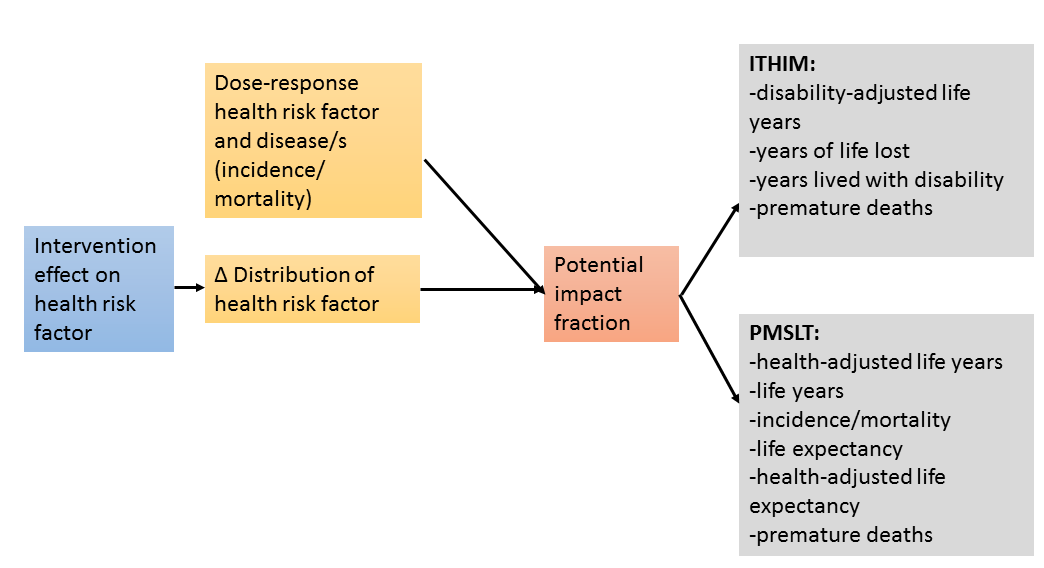
\includegraphics{structure/Figure1.png}

\textbf{HALYs, QALYs and DALYs}

In this model we use the term `health-adjusted life year' (HALY). As
`summary measure of population health' it measures both quantity and
quality of life, where one HALY represent the equivalent of one year in
full health (which could be two years with a quality of life of 0.5, for
example). Specific types of HALY are the quality-adjusted life year
(QALY) and the disability-adjusted life year (DALY). The QALY derives
from economics and was first used in the 1960s as a measure of health
gain (Gold, Stevenson, and Fryback 2002). The disability-adjusted
life-year (DALY) was developed for use in burden of disease studies as a
measure of health loss due to disease (Gold, Stevenson, and Fryback
2002). Our calculated HALYs are neither QALYs not DALYs, but something
in between. They are similar to QALYs in that they represent health
gains. However, the main difference is in the calculation of the
health-related quality of life component. QALYs use measures of utility
weights that traditionally represent individual experiences of health,
whereas our estimated HALYs use disability weights linked to specific
diseases, which were developed for the Global Burden of Disease study
(Gold, Stevenson, and Fryback 2002). As discussed in past research (L.
Cobiac, Vos, and Barendregt 2009; Roux, Pratt, and Tengs 2008) the main
advantage of using disability weights over utility weights is that
disability weights refer to specific diseases rather than health states.
We opted to use the more general terms HALYs given that the use of the
DALYs terminology may lead to think that our calculations are similar to
those in burden of diseases studies (Murray et al. 2012). In our study,
our model does not explicitly separate years of life lost (YLL) and
years lived with disability (YLD) components, but instead calculates the
total number of life years lived, adjusted for the average
health-related quality of life in those years (by age and sex). In
burden of disease studies, DALYs are defined as the sum Years of Life
Lost (YLL) and Years Lived with Disability (YLD).

\subsection{Contribution to ITHIMR}\label{contribution-to-ithimr}

The PMSLT similar to ITHIM is a comparative risk assessment approach
(Briggs, Scarborough, and Smith 2016) that consist of calculating the
change in the health burden for a population of interest from a change
in exposure to health risks factors (e.g.~physical inactivity, air
pollution and road trauma).As depicted in Figure 1, both methods need
estimates of the potential impact fraction (PIF), which indicates the
proportion of the disease burden attributable to a risk factor of
interest (e.g.~physical inactivity) (Barendregt and Veerman 2010). A
step further back, is the development of scenarios that bring about
change in the distribution of the risk factor of interest. For now, we
only focus on calculations from the PIF onward, and provide a
hypothetical example of change in population levels of physical
activity. Incorporation of additional health risk factor (air pollution,
road trauma, NO2 and noise) will be discussed in the relevant code
sections.

\subsubsection{Difference between ITHIM and
PMSLT}\label{difference-between-ithim-and-pmslt}

\begin{itemize}
\item
  \textbf{Time component} The \emph{PMSLT} follows a population of
  interest over time. For example, as set up here, we simulate sex and
  age (5 years starting at 18) cohorts over time until they die or reach
  100 years of age. This implies that we can include trends for
  diseases, time lags between change in exposure to risk factors and
  change in health and demographic changes (e.g.~population growth). In
  addition, we can estimate yearly changes in the burden of diseases
  over the life course or for a specified number of years. The
  \emph{ITHIM} approach is a snapshot of change in burden for one year.
\item
  \textbf{Interaction between multiple diseases} The \emph{PMSLT}
  accounts for the interaction between multiple diseases, with
  proportions of the population being able to be in more than one health
  state (Briggs, Scarborough, and Smith 2016). This avoids
  overestimation of outcomes as a result of summing health outcomes
  attributable to each disease individually as done in \emph{ITHIM}. It
  is important to note that the \emph{PMSLT} assumes that diseases are
  independent of each other. That is to say, developing a disease is
  unrelated to a concurrent diagnoses of another disease).
\item
  \textbf{Mortality rate} The \emph{PMSLT} calculations for changes in
  life years (and health-adjusted life years) and mortality outcomes is
  based on observed mortality rates for the population of interest. In
  the \emph{ITHIM} model, if burden of disease estimates from the Global
  Burden of Disease (GBD) study are used, then, the mortality component
  is based on the highest attained life expectancy observed in the
  world.
\item
  \textbf{Impact of disability in increased life expectancy} In GBD
  studies, YLLs are not adjusted for disability; hence, their use in
  estimating intervention effects results in over-estimation, which the
  \emph{PMSLT} approach avoids. Another way of seeing this is that
  estimated changes in morbidity using the \emph{ITHIM} do not allow for
  how implicit increases in life expectancy impact on morbidity. While
  the changes in deaths and prevalence using the \emph{PMSLT} are in
  some ways more accurate than those from the \emph{ITHIM} approach it
  should be noted that that the average age of death and incident
  disease will change and thus the disease burden will be on average be
  shifted later in life (which is a realistic approach).
\end{itemize}

\section{R development}\label{r-development}

The model is set up as a long script to perform the required
mathematical calculations. Where possible, we wrote functions and loops
to avoid repetition. We set up the model with Australian data, for
Melbourne. Figure 2 is depicts the PMSLT model framework, which was
followed in the code development.

\begin{figure}
\centering
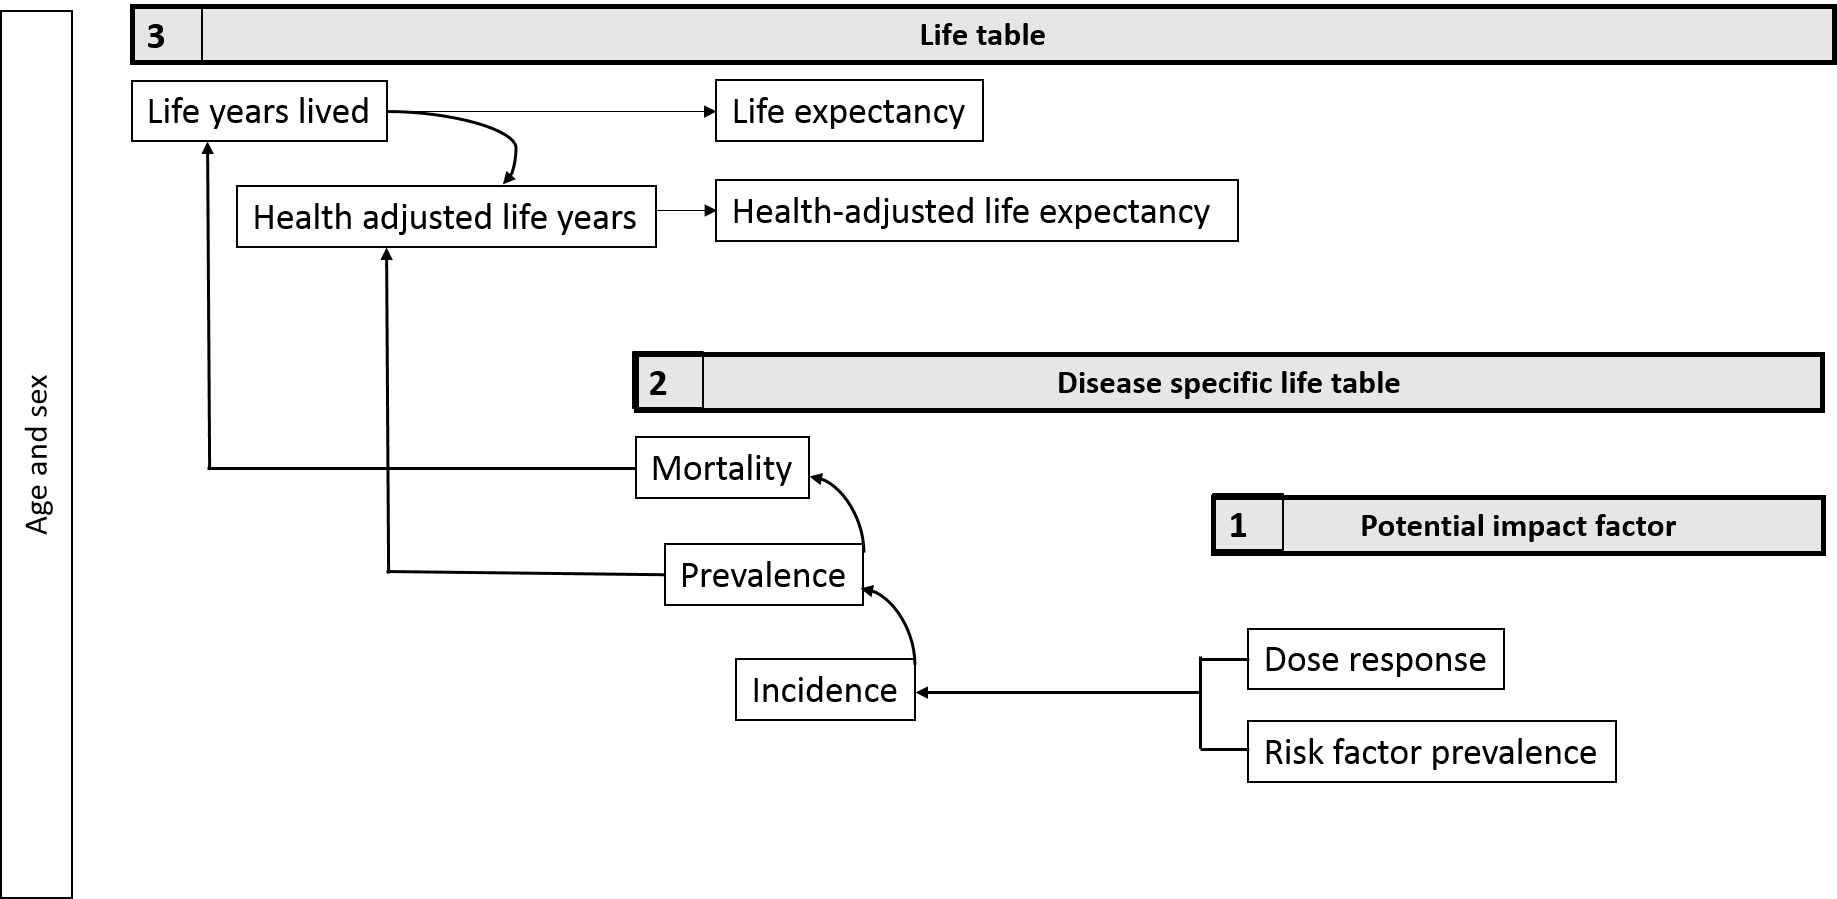
\includegraphics{structure/Figure2.png}
\caption{Figure 2. Proportional multi-state life-table simplified
framework. \emph{The simplied PMST shows the interaction between the
life table, disease life table and potential impact fraction (PIF). The
PIF calculations by age and sex group are the same as those generated
for ITHIM. The PIF (or 1-PIF) modifies incidence of disease, which
changes prevalence and mortality (disease specific life table). Changes
in prevalence and mortality rates from the disease specific life tables
feed into the life table by changing all-cause mortality, which in turn
changes life years. Change in prevalence of diseases changes total years
lived with disability, which in turn modifies health-adjusted life
years}}
\end{figure}

In what follows, first, we specify input parameters. Second, we present
the code with explaining notes. Third, we present examples of outcomes
and lastly we comment on topics related to implementation. Here we only
included the physical activity health pathway. In the comments section,
implementation of exposure to air pollution and road trauma is
discussed. Note that in the presentation of input parameters, those
needed to calculate PIFs are excluded, as these are common to the ITHIM,
expect if trends are included (refer to comments section).

\subsection{Inputs}\label{inputs}

We specify data requirements for the life table and disease life tables
(Figure 2) and potential sources.

\subsubsection{\texorpdfstring{\textbf{Life
table}:}{Life table:}}\label{life-table}

Inputs of the life table are: population numbers by sex (per 1-year or
age grouping of interest), mortality rates or probability of all cause
mortality by single age group and sex and total prevalent years lived
with disability rate per one year by sex.

\paragraph{Population numbers}\label{population-numbers}

These data will be provided by the synthetic population. In the code
presented here, we created 5-year age and sex cohorts from one-year age
groups data. I left potential data sources below as a reference.

Data source: (1) National census; (2) Worldwide population and mortality
data: \url{http://www.mortality.org/} (mostly high income countries; and
(3) Calculate from GBD data (rates and numbers).

\paragraph{Mortality rates}\label{mortality-rates}

These data will be provided by the synthetic population. Other sources
are the same sources as above for population numbers. Sometimes
mortality rates are in age groups (1-4, 5-9, etc). Interpolation can be
used to derive in between ages rates (cubic spline). Here, mortality
rates are needed per single year and sex.

Note that we need data for population numbers and all cause mortality
rates for: (1) PMSLT and (2) Dismod II collection (more in Dismod II
section).

\paragraph{Total years lived with disability rates per single year and
sex.}\label{total-years-lived-with-disability-rates-per-single-year-and-sex.}

These data is available from the GBD
(\url{http://ghdx.healthdata.org/gbd-results-tool}) per 5-year age
groups. We can use interpolation to derive between ages rates.

\subsubsection{\texorpdfstring{\textbf{Disease life
tables}}{Disease life tables}}\label{disease-life-tables}

\paragraph{Incidence and case
fatality}\label{incidence-and-case-fatality}

For each of the modeled diseases the PMSLT needs incidence and case
fatality rates per sex and one-year intervals. Data from the GBD studies
with Dismod II (free at
\url{https://www.epigear.com/index_files/dismod_ii.html}) can be used to
derive internally consistent data and generate missing data. For
example, the GBD studies provide data for incidence, prevalence and
disease mortality, however, not case fatality. Other national level
sources may also be explored/used, and compare with estimates produce
from GBD data and Dismod II.

\textbf{Dismod II} inputs are: (1) population numbers and mortality
rates and (2) disease specific inputs.

\emph{Population and mortality}

Within Dismod II, each setting (e.g.~country) has a collection that
consists of population numbers (preferably the same as used in GBD
studies, due to the mortality envelop) and all- cause mortality rates
(numbers and calculate rates). The GBD provides 5-year age groups that
are acceptable input parameters for Dismod II.

\emph{Disease inputs by age group and sex}

Each setting collection has a given number of diseases. Dismod II works
with at least three of: case fatality, prevalence, incidence, mortality
(disease), case fatality, remission, duration and the relative risk for
mortality. So far, we have been assuming that remission is zero for
chronic diseases, that is to say, when people become diseased, they do
not recover. Special care should be taken with this assumption, as the
GBD data assumes remission for some diseases, for example cancers, where
after 10 years cases recover, except for long term sequelae. Since GBD
now provides prevalence, incidence and mortality, it may be best to use
all three as Dismod II input parameters to compare the effect of the
remission assumption by the GBD for some diseases.

\paragraph{Disability weights (quality of life
weights)}\label{disability-weights-quality-of-life-weights}

Disability weights (DW) can be derived from disease specific years lived
with disability (YLD) and disease specific prevalence by age group (5
years) and sex. Data for YLDs prevalence can be obtained from the online
GBD data tool (\url{http://ghdx.healthdata.org/gbd-results-tool}). Our
calculations of DW in the example here based on the GBD methods for
estimating YLDs as the sum of sequelae prevalence multiplied by sequelae
disability weights (REF GBD). The GBD has publicly available data at the
cause level (e.g.~ischemic heart disease) instead of squelae level
(e.g.~myocardial infarction, angina and heart failure). However, the GBD
disability weights are for health states associated with sequelae,
hence, we need to calculate DWs. An age and sex specific-correction was
introduced to counteract the effects of accumulating comorbid illnesses
in the older age groups (Equation 1).

\begin{equation}
\label{DW adjusted for total YLDs-YLDdPd1YLDt}
(YLDd/Pd)/(1-YLDt) = DW adjusted for total YLDs
\end{equation}

Where YLDd is the YLD mean number per age and sex for a given disease,
Pd is the prevalence (as reported in GBD ) for a given disease by age
and sex and YLDt is total YLD rate per age and sex.

\rowcolors{2}{gray!6}{white}

\begin{table}

\caption{\label{tab:unnamed-chunk-1}PMSLT inputs}
\centering
\begin{tabular}[t]{l>{\raggedright\arraybackslash}p{15em}>{\raggedright\arraybackslash}p{15em}}
\hiderowcolors
\toprule
\textbf{Input} & \textbf{Source} & \textbf{Comments}\\
\midrule
\showrowcolors
Life table & Synthetic population per sex and age group & Age grouping in life table to match synthetic population\\
Life table & Synthetic population per sex and one-year age group & If one year age group is not avabilable it can be derive using interpolation from age groups data\\
Life table & Global Burden of Disease (GBD) study per one-year age group and sex & GBD data is in five-year age groups, interpolation to derive one-year age groups\\
Disease life table & GBD data for prevalence, incidence and mortality and DISMOD II & Two step process. First obtain disease and population data from GBD. Second, use Dismod II to derive internally consistent estimates for incidence and case fatality (PMSLT disease life table iputs\\
Disease life table & Derive from disease prevalence and years lived with disability from GBD & Adjustments for comorbidities in later years of life to be applied\\
\bottomrule
\end{tabular}
\end{table}

\rowcolors{2}{white}{white} \pagebreak

\subsection{Code}\label{code}

Following the structure of Figure 2, we developed functions to perform
sex and age cohorts calculations for the life table, disease life tables
and potential impact fractions: run\_life\_table, run\_disease and and
run\_pif. We also generated two functions for outputs: plot\_outputs and
gen\_aggregate. The function plot\_outputs creates age-group and sex
linear plots for specified outcomes (e.g.~health-adjusted life years,
incidence of diabetes) and gen\_aggregate adds up each cohort results.
Functions were then used in a code script. In what follows, we explain
each step in the development of the script. Here we also include code
chunks, however, we also kept them separately in the MSLT folder, in the
code file.

In what follows, we start with the \textbf{mode} script file, and
explain the \textbf{functions} script file as these are used to perform
calculations. The \textbf{functions} will be explained in detailed to
provide clarity for required inputs.

\subsection{Including Plots}\label{including-plots}

You can also embed plots, for example:

\includegraphics{MSLTdoc_files/figure-latex/pressure-1.pdf}

Note that the \texttt{echo\ =\ FALSE} parameter was added to the code
chunk to prevent printing of the R code that generated the plot.

\section{Comments}\label{comments}

\subsection{Road injuries in the
PMsLT}\label{road-injuries-in-the-pmslt}

The disease model used in each of the disease life table is not directly
applicable to road injuries, however, similar concept can be follow.
Firstly, changes in road fatalities impact on the overall mortality
rate, hence, by knowing the road fatality rates for baseline and
scenarios, we will be able to incorporate changes to mortality
attributable to road fatalities. For road injuries, methods developed by
Kavi Bhalla and Marko Tanio (REFS) that derive the average YLD
attributable to life long and short term injuries can be applied to
derive the change in total YLDs (CHECK THAT THESE WERE DEVELOPED AS
INCIDENCE YLDs).MT's methods assumes that injuries do not reduce the
life expectancy of the injured person.

\section*{References}\label{references}
\addcontentsline{toc}{section}{References}

\hypertarget{refs}{}
\hypertarget{ref-RN42}{}
Barendregt, J.J., and J.L. Veerman. 2010. ``Categorical Versus
Continuous Risk Factors and the Calculation of Potential Impact
Fractions.'' Journal Article. \emph{J Epidemiol Community Health} 64
(3): 209--12.
doi:\href{https://doi.org/10.1136/jech.2009.090274}{10.1136/jech.2009.090274}.

\hypertarget{ref-RN8299}{}
Blakely, T., L. J. Cobiac, C. L. Cleghorn, A. L. Pearson, F. S. Deen, G.
Kvizhinadze, N. Nghiem, M. McLeod, and N. Wilson. 2015. ``Health, Health
Inequality, and Cost Impacts of Annual Increases in Tobacco Tax:
Multistate Life Table Modeling in New Zealand.'' Journal Article.
\emph{PLoS Med} 12.
doi:\href{https://doi.org/10.1371/journal.pmed.1001856}{10.1371/journal.pmed.1001856}.

\hypertarget{ref-RN8957}{}
Briggs, Adam, Peter Scarborough, and Adrian Smith. 2016. ``Modelling in
Public Health.'' Book Section. In \emph{Public Health Intelligence:
Issues of Measure and Method}, edited by Krishna Regmi and Ivan Gee,
67--90. Cham: Springer International Publishing.
doi:\href{https://doi.org/10.1007/978-3-319-28326-5_4}{10.1007/978-3-319-28326-5\_4}.

\hypertarget{ref-RN21}{}
Cobiac, L.J., T. Vos, and J.J. Barendregt. 2009. ``Cost-Effectiveness of
Interventions to Promote Physical Activity: A Modelling Study.'' Journal
Article. \emph{Plos Med} 6 (7): e1000110--e1000110.
doi:\href{https://doi.org/10.1371/journal.pmed.1000110}{10.1371/journal.pmed.1000110}.

\hypertarget{ref-RN8158}{}
Gold, Marthe R., David Stevenson, and Dennis G. Fryback. 2002. ``HALYs
and Qalys and Dalys, Oh My: Similarities and Differences in Summary
Measures of Population Health.'' Journal Article. \emph{Annu Rev Public
Health} 23 (1): 115--34.
doi:\href{https://doi.org/doi:10.1146/annurev.publhealth.23.100901.140513}{doi:10.1146/annurev.publhealth.23.100901.140513}.

\hypertarget{ref-RN8153}{}
Murray, Christopher J. L., Majid Ezzati, Abraham D. Flaxman, Stephen
Lim, Rafael Lozano, Catherine Michaud, Mohsen Naghavi, et al. 2012.
``GBD 2010: Design, Definitions, and Metrics.'' Journal Article.
\emph{The Lancet} 380 (9859): 2063--6.
doi:\href{https://doi.org/10.1016/S0140-6736(12)61899-6}{10.1016/S0140-6736(12)61899-6}.

\hypertarget{ref-RN8262}{}
Roux, L., M. Pratt, and T. O. Tengs. 2008. ``Cost Effectiveness of
Community-Based Physical Activity Interventions.'' Journal Article.
\emph{Am J Prev Med} 35.
doi:\href{https://doi.org/10.1016/j.amepre.2008.06.040}{10.1016/j.amepre.2008.06.040}.

\hypertarget{ref-RN38}{}
Vos, T., R. Carter, J. J Barendregt, Mihalopoulos C., JL. Veerman, A.
Magnus, L. Cobiac, Bertram MY., and AL. Wallace. 2010. ``Assessing
Cost-Effectiveness in Prevention (Ace-Prevention): Final Report.''
Report.


\end{document}
